\videotitle{Search Spaces}

%-------------------------------------------------
%-------------------------------------------------

%-----------------------------------------------------------------------
\myframe{Basic Neural Architecture Search Spaces}{
\centering
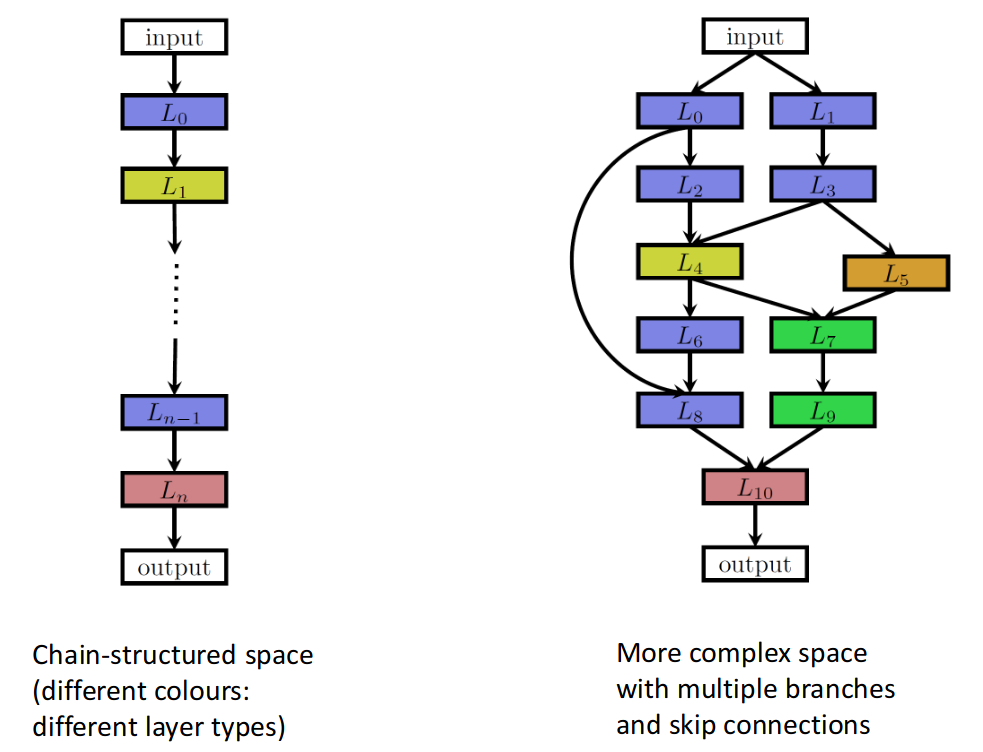
\includegraphics[height=0.9\textheight]{images/macro_space.png}
}
%----------------------------------------------------------------------

%----------------------------------------------------------------------
\myframe{Cell Search Spaces \litw{\href{https://openaccess.thecvf.com/content_cvpr_2018/papers/Zoph_Learning_Transferable_Architectures_CVPR_2018_paper.pdf}{Zoph et al. 2018}}}{
\centering
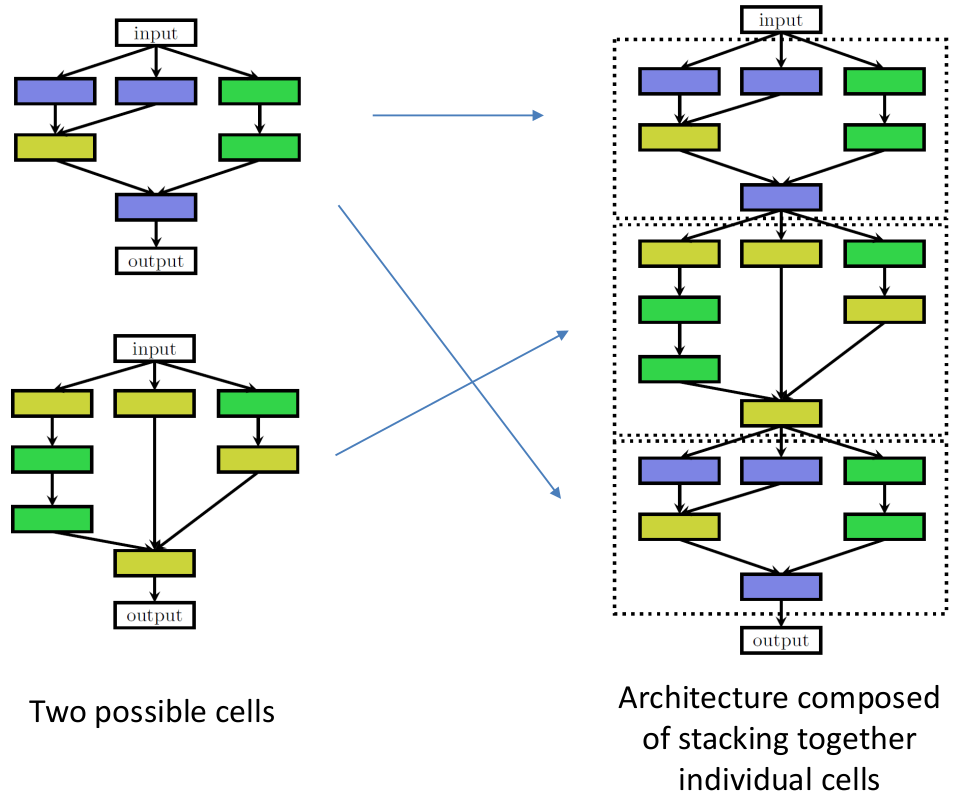
\includegraphics[height=.8\textheight]{images/s26}
}
%----------------------------------------------------------------------

%----------------------------------------------------------------------

\myframetop{Details on Cell Search Spaces \litw{\href{https://openaccess.thecvf.com/content_cvpr_2018/papers/Zoph_Learning_Transferable_Architectures_CVPR_2018_paper.pdf}{Zoph et al. 2018}}}{
	\centering
	
	\begin{itemize}
		\item 2 types of cells: normal and reduction cells
		\item For each type of cell: $B$ blocks, each with 5 choices
		\myit{
			\item[-] Choose two previous feature maps (from this cell)
			\item[-] For each of these, choose an operation (3$\times$3 conv, max-pool, etc.)
			\item[-] Choose a merge operation to combine the two results (concat or add)
		}
	
	\end{itemize}
	\bigskip
	\bigskip
	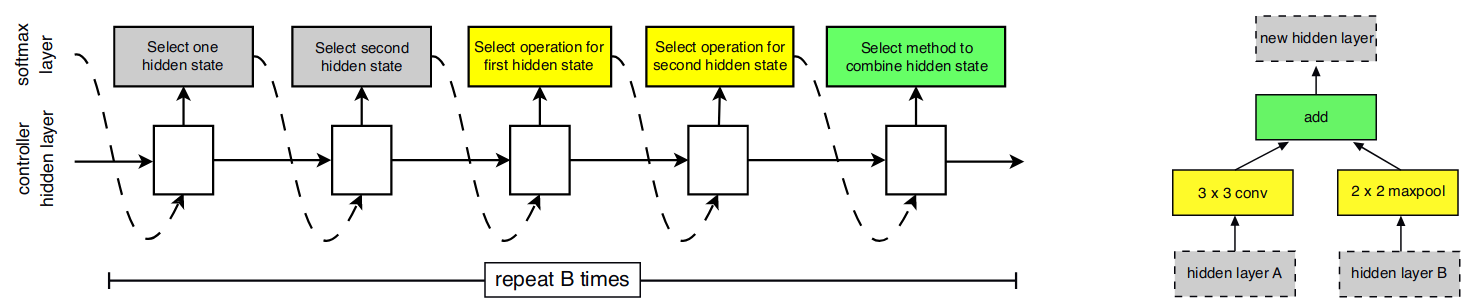
\includegraphics[width=\textwidth]{images/RL_conv_cell}
	%\pause
	%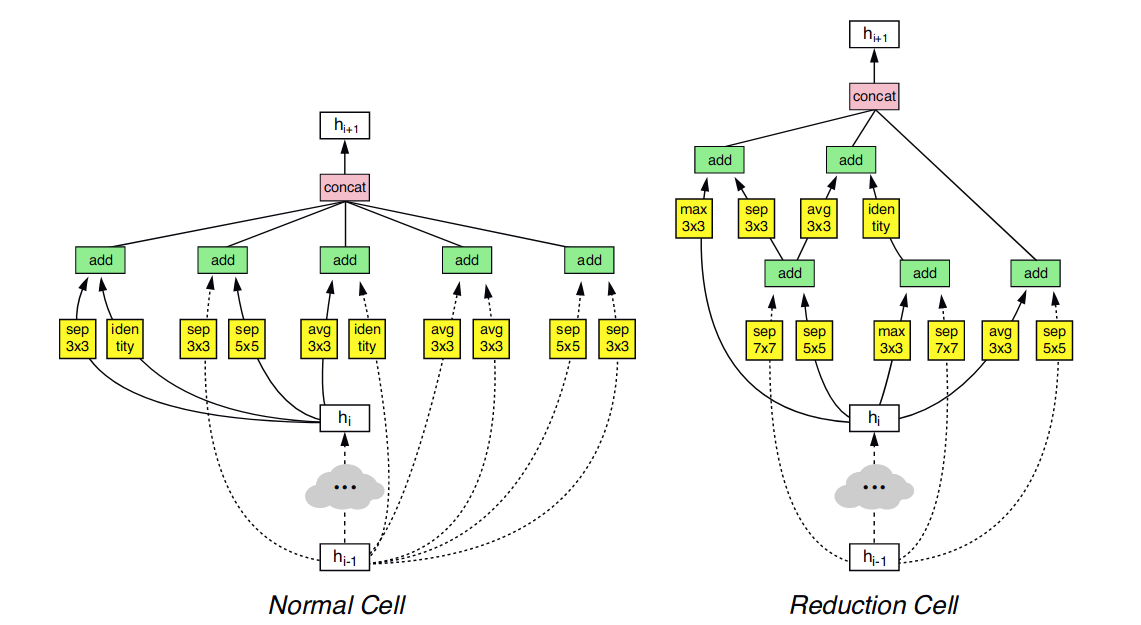
\includegraphics[width=.5\textwidth]{images/RL_normal_reduction}
	
}
%----------------------------------------------------------------------

%----------------------------------------------------------------------
\myframetop{Example of an architecture sample with B=5}{
\centering
\begin{columns}
	\column{0.3\textwidth}
	\centering
	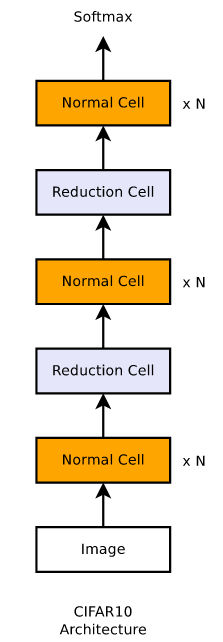
\includegraphics[width=.5\textwidth]{images/nasnet_full_net.png}

%\vspace{5cm}	
	\column{0.68\textwidth}
	\centering
	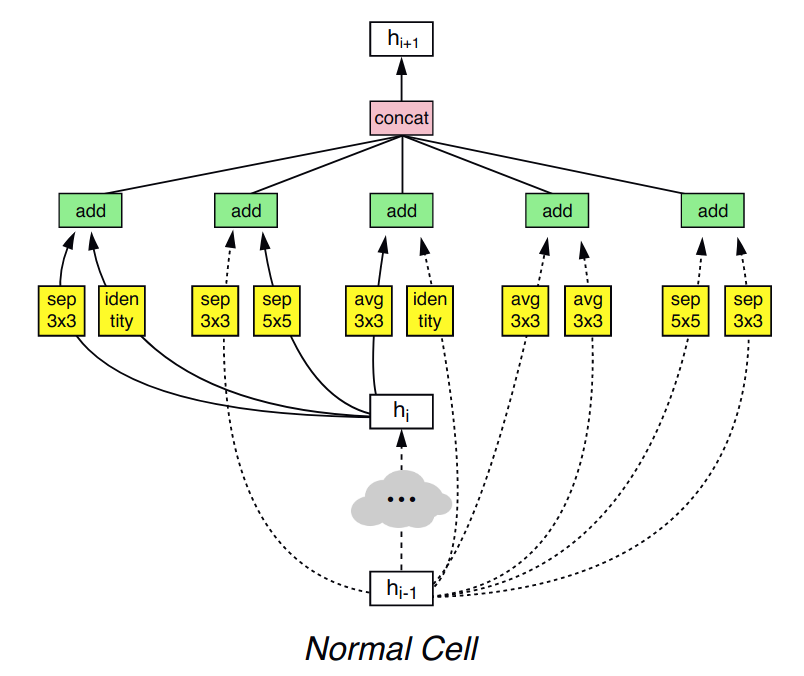
\includegraphics[width=.47\textwidth]{images/nasnet_normal.png}
	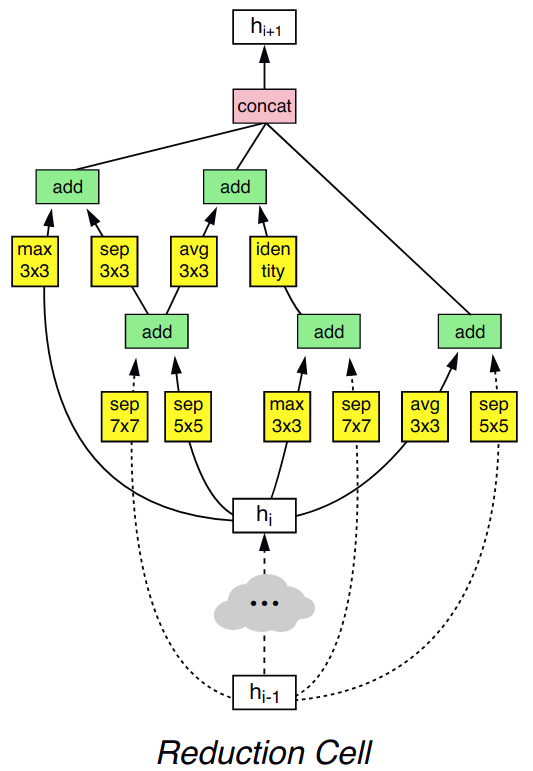
\includegraphics[width=.35\textwidth]{images/nasnet_reduce.png}
\end{columns}

\centering
Source: \lit{\href{https://openaccess.thecvf.com/content_cvpr_2018/papers/Zoph_Learning_Transferable_Architectures_CVPR_2018_paper.pdf}{Zoph et al. 2018}}
}
%----------------------------------------------------------------------

%----------------------------------------------------------------------
\myframe{Pros and Cons of Cell Search Space}{
\centering
What are some pros and cons of the cell search space compared to the basic one?\\~\\
Please think about this for a few minutes before continuing.
}
%----------------------------------------------------------------------

%----------------------------------------------------------------------
\myframe{Pros and Cons of Cell Search Space}{
\centering
\alert{Pros:}
\begin{itemize}
	\item Reduced search space size; speed-ups in terms of search time.
	\item Transferability to other datasets (e.g., cells found on
	CIFAR-10 transfer to ImageNet)
	\item Stacking repeating patterns is proven to be a useful design principle 
	(ResNet, Inception, etc.)
\end{itemize}
\pause
\medskip
\alert{Cons:}
\begin{itemize}
	\item Still need to (manually) determine the \textit{macro} architecture, 
	i.e., the way in which cells are connected.
	\item Limiting if different cells work better in different parts of the network
	\myit{
		\item[-] E.g., different spatial resolutions may favour different convolutions
	}
%	, e.g., different cells would be best at the beginning and end of the network.
\end{itemize}

}
%----------------------------------------------------------------------

%----------------------------------------------------------------------
\myframe{Hierarchical representation of search space \litw{\href{https://openreview.net/pdf?id=BJQRKzbA-}{Liu et al. 2017}}}{
	\centering
	\myit{
		\item Directed Acyclic Graph (DAG) representation of architectures
		\myit{
			\item[-] Each node is a latent representation; each edge is an operation/motif
		}
	\medskip		
	\pause
		\item There are different \alert{levels} of motivs
		\myit{
%			\item E.g. $o_1^{(2)}$ is a level-2 motif, $o_1^{(3)}$ is a level-3 motif
			\item \alert{Level-1 primitives}: standard operators; e.g., 3x3 conv, max pooling, \ldots
	\medskip		
	\pause
			\item \alert{Level-2 motivs}: combinations of level-1 primitives
		} 
	\centering
	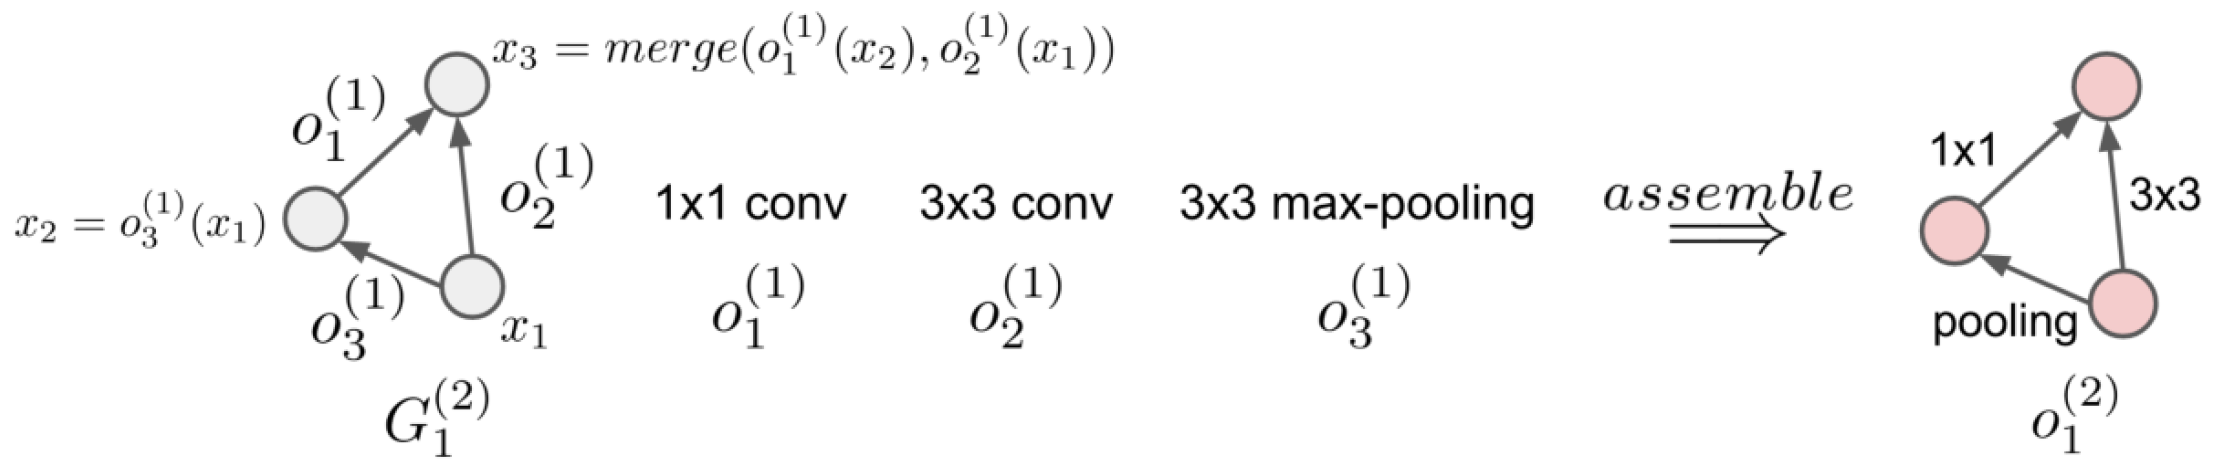
\includegraphics[width=0.6\textwidth]{images/hierarchical_nas_level1_2.png}
	\medskip		
	\pause
		\myit{
			\item \alert{Level-3 motivs}: combinations of level-2 motivs
		}
	\centering
	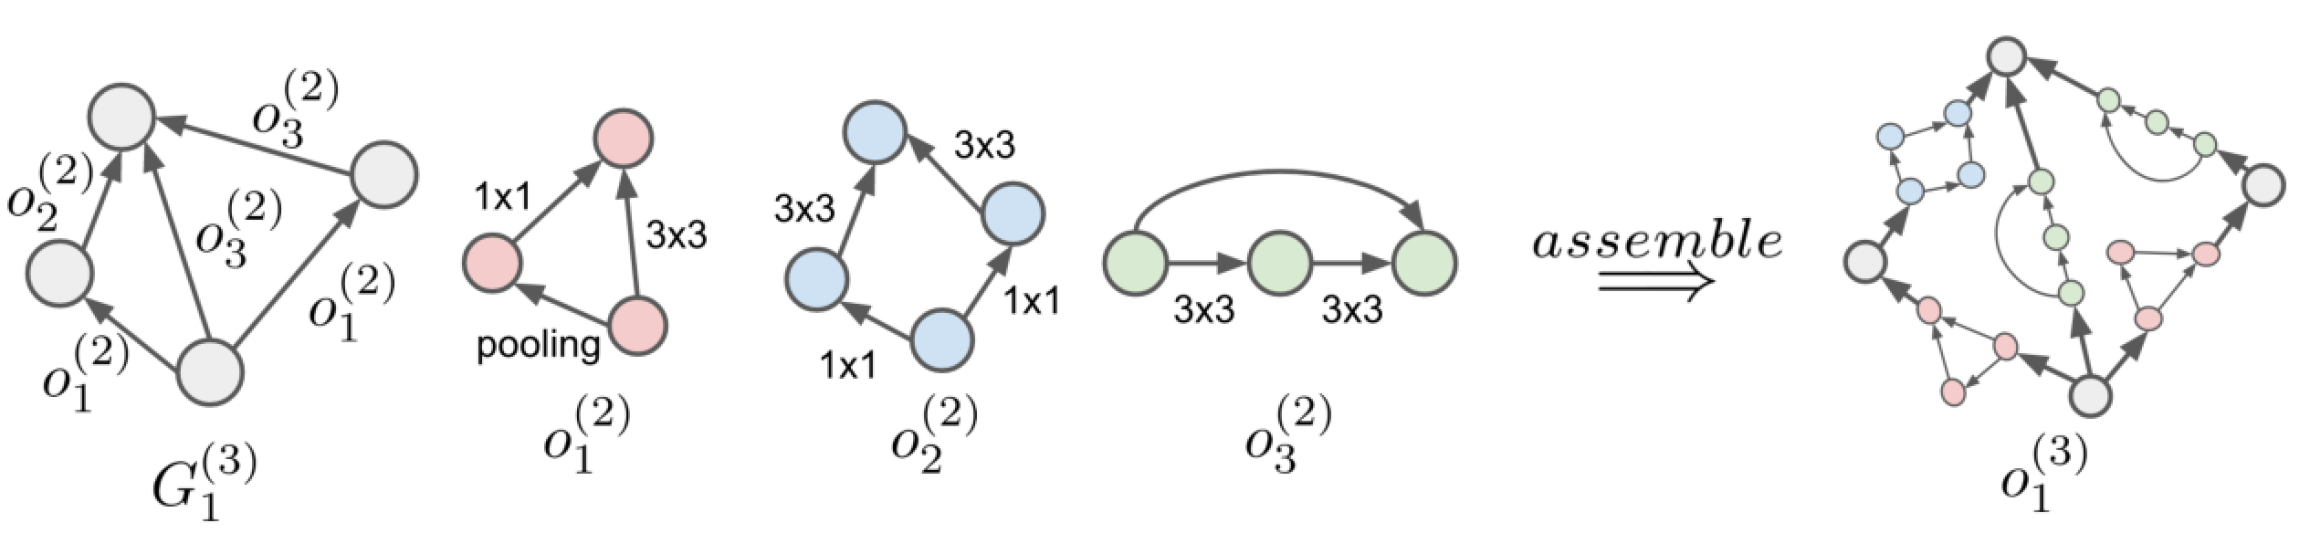
\includegraphics[width=0.6\textwidth]{images/hierarchical_nas_level2_3.png}
	}
%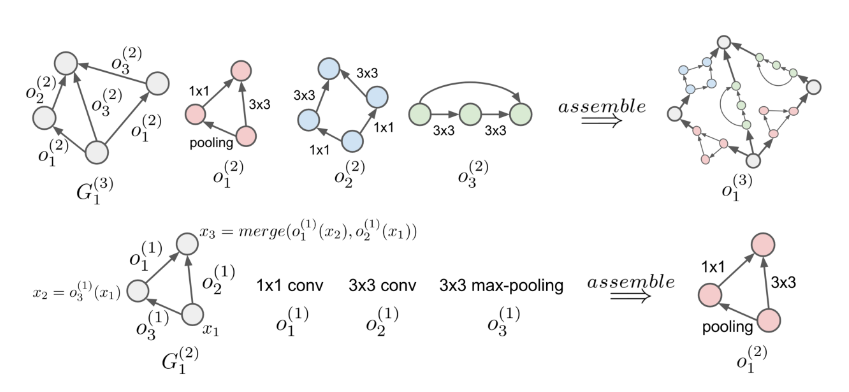
\includegraphics[width=\textwidth]{images/hierarchical_nas.png}\\
}
%----------------------------------------------------------------------

%----------------------------------------------------------------------
\myframe{Pros and Cons of Hierarchical Search Space}{
\centering
What are some pros and cons of a hierarchical search space compared to the cell search space?\\~\\
Please think about this for a few minutes before continuing.
}
%----------------------------------------------------------------------

%----------------------------------------------------------------------
\myframe{Pros and Cons of Hierarchical Search Space}{
	\centering
	\alert{Pros:}
	\begin{itemize}
		\item \alert{Flexibility} of \alert{constructing building blocks and reusing them many times}
		\myit{
			\item like a cell search space
		}
		\item \alert{Flexibility} of using different building blocks in different parts of the network
		\myit{
			\item like a basic search space
		}
		\item Ability to \alert{reuse building blocks at various levels of abstraction}
		\myit{
			\item again, this pattern has been used in manual design, e.g., in Inception nets
		}
	\end{itemize}
	\pause
	\bigskip
	\alert{Cons:}
	\begin{itemize}
		\item \alert{Larger} than cell search space
		\item Vastly more expressive than cell search space $\rightarrow$ \alert{potentially much harder to search}
	\end{itemize}
}
%----------------------------------------------------------------------


%----------------------------------------------------------------------
\myframe{Questions to Answer for Yourself / Discuss with Friends}{

	\myit{
		\item Repetition:\\ \alert{What are some pros and cons of the cell search space compared to the basic one?}
\bigskip
		\item Repetition:\\ \alert{Explain the way in which level-3 motivs in the hierarchical search space use level-2 motivs.}
\medskip
		\item Repetition:\\ \alert{What are some pros and cons of the hierarchical search space compared to the other ones?}
	}	 
}
%-----------------------------------------------------------------------


